%%%%             %%%%
%%%% ADICIONAL 2 %%%%
%%%%             %%%%

\chapter{Material adicional}
\label{chap:material-adicional}

\section{Textract y Document AI}

Dos servicios diferentes a los productos mencionados en el Capítulo \ref{chap:estado-arte} pero aplicables al problema son, Textract de Amazon \cite{solucionesComerciales_amazon_textract} y Document AI de Google \cite{solucionesComerciales_google_documentAI}. Ninguno de los dos suporta el flujo de información explicado ni están pensados para ser solución para el usuario final. Lo que ofrecen es un \emph{\acrshort{api}} capaz de recibir documentos y generar información estructurada como salida. El caso de Textract es totalmente opaco y por tanto no configurable. La salida consiste en ficheros JSON donde puede haber varios tipos de objetos: páginas, líneas y palabras, información de formularios (pares clave-valor), tablas, y elementos seleccionables como casillas. Además es capaz de identificar notas manuscritas. El servicio de Google permite definir \emph{processors}, que son plantillas específicas para modelos de documentos concretos. Actualmente parece que el servicio es muy reciente y está mayormente en beta. Cualquiera de ellos podría utilizarse para construir una solución más completa. Como otros servicios en la nube, el coste depende de la carga de trabajo procesada.

\section{Instalación de software}
\label{chap:instalacion-software}

La instalación completa desde el código fuente implica la descarga del contenido presente en el repositorio git.

En esta sección se asume que se utilizará una distribución Ubuntu 18.04 igual a la empleada durante el desarrollo. Para la correcta compilación y ejecución es necesario que varias aplicaciones y librerías estén disponibles en el sistema. En el caso de las nuevas versiones de Ubuntu, la lista de paquetes a instalar no presentará diferencias pero si se utiliza Fedora u otras será necesario averiguar que paquetes contienen el software utilizado e instalarlos.

Se pueden distinguir dos escenarios distintos. Los requisitos necesarios para compilar los fuentes y aquellos imprescindibles únicamente para ejecutar la aplicación. Para el primer caso se debe utilizar el comando mostrado en \ref{lst:requisitos-para-compilacion}. El paquete \verb|build-essential| instala la mayor parte de las aplicaciones como el compilador de C y Make.

\begin{lstlisting}[language=bash,caption={Dependencias para la compilación.},label=lst:requisitos-para-compilacion]
    sudo apt-get build-essential libpcre2-dev bison flex
\end{lstlisting}

En el caso de tener ya la aplicación compilada y empaquetada, será necesarios instalar los componentes para la ejecución, como Tesseract, el software de OCR. La orden del listado \ref{lst:requisitos-para-ejecucion} instalará estos requisitos.

\begin{lstlisting}[language=bash,caption={Dependencias para la ejecución.},label=lst:requisitos-para-ejecucion]
    sudo apt-get install unzip poppler-utils mediainfo tesseract-ocr tesseract-ocr-spa jq python3-opencv jq bc
\end{lstlisting}

De manera opcional, pero recomendable, se puede utilizar un PPA específico para obtener una versión actualizada de Tesseract. Un PPA en el entorno Ubuntu, es un repositorio personal, en este caso mantenido por Alexander Pozdnyakov \footnote{\url{https://launchpad.net/~alex-p/+archive/ubuntu/tesseract-ocr}}. La activación de este repositorio debe hacerse previamente a la instalación del software. En necesario ejecutar los comandos del listado \ref{lst:activar-ppa-tesseract}.

\begin{lstlisting}[language=bash,caption={Activar PPA de Tesseract.},label=lst:activar-ppa-tesseract]
    sudo add-apt-repository ppa:alex-p/tesseract-ocr
    sudo apt-get update
\end{lstlisting}

No se ahondará en el uso del software ya que ha sido explicado en detalle en el capítulo \ref{chap:implemetación}.

\section{Visor del formato hOCR}

Existen herramientas para trabajar con el formato hOCR, por ejemplo en el repositorio git del proyecto OCRopus \footnote{\url{https://github.com/ocropus/hocr-tools}} pero si lo que se quiere es poder ver una superposición de las líneas y regiones definidas para una página, el Pattern Recognition \& Image Analysis Research Lab de la Universidad de Salford mantiene una utilidad para hacer justo esto \cite{prima_tool_page_viewer}. En la imagen \ref{fig:visor-formato-hocr} el visor muestra las líneas detectadas para una página del proveedor AC. Además de hOCR la herramienta soporta otros formatos.

\begin{figure}[hp!]
    \centering
    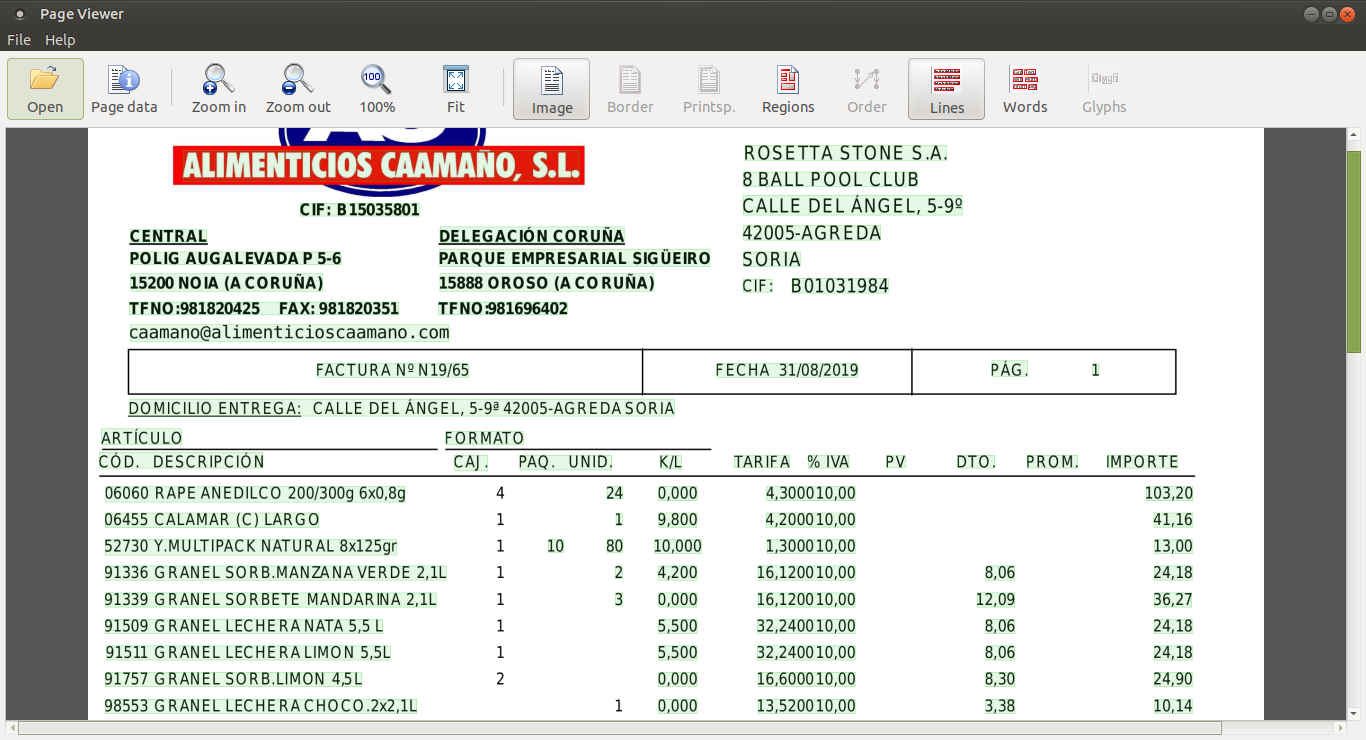
\includegraphics[width=1.0\textwidth]{imaxes/z-adicional/visor-hocr.png}
    \caption{Visor del formato hOCR con un documento de AC.}
    \label{fig:visor-formato-hocr}
\end{figure}

\section{Ansible}

% TODO Presentar Ansible y mostrar el script desarrollado

Ansible es una tecnología para automatizar administración y la configuración de ordenadores. Fue creado inicialmente en el año 2012 por Michael DeHaan, hoy en día forma parte del catálogo de productos de Red Hat.

\begin{wrapfigure}{R}{0.3\textwidth}
    \centering
    
\includegraphics[width=0.25\textwidth]{imaxes/e-fundamentos-tecnologicos/logo-ansible.png}
\end{wrapfigure}

Ansible es una tecnología del ámbito de la Gestión de la Configuración. Durante los años 50 el Departamento de Defensa de los Estados Unidos tenía necesidad de crear una metodología para mantener el inventario de los recursos materiales. La Gestión de la Configuración es aquel conjunto de procesos que permiten gestionar los cambios en un sistema utilizando un método conocido de tal manera que se mantenga la integridad del sistema a lo largo del tiempo. La manera de conseguirlo es llevando un registro de los cambios a los que a sido sometido y se consigue conocer cual es el estado actual y como se ha llegado esta este estado. MÉTRICA v3 es un ejemplo de sistema español para la Gestión de la Configuración.

Estas ideas se comenzaron a aplicar a los ordenadores para llevar registro tanto del hardware como de los Sistemas Operativos y aplicaciones instaladas. Gracias al avance y aparición de tecnologías como Ansible, en lugar de generar documentos describiendo los estados se pasa directamente a especificar cuales son los estados deseados y la herramienta realiza los cambios necesarios para asegurar que el estado alcanzado sea el correcto tras la intervención.

Ansible está escrito en Python y su funcionamiento es simple. Para realizar la gestión conecta a las máquinas por SSH y aplica los cambios indicados en los ficheros conocidos como Playbooks. Estos ficheros son guiones escritos en YAML que indican a Ansible las acciones a acometer. La sintaxis de YAML guarda parecidos con Markdown y es fácil de comprender.

En el Listado \ref{lst:ejemplo-playbook} se muestra un Playbook mínimo que da instrucciones a Ansible para realizar un ping a todos los anfitriones definidos.

\begin{lstlisting}[language=Python,caption={Ejemplo mínimo de Playbook.},label=lst:ejemplo-playbook]
    ---
    - hosts: all
    tasks:
    - ping:
\end{lstlisting}